% Digital Logic Report Template
% Created: 2020-01-10, John Miller

%==========================================================
%=========== Document Setup  ==============================

% Formatting defined by class file
\documentclass[11pt]{article}

% ---- Document formatting ----
\usepackage[margin=1in]{geometry}	% Narrower margins
\usepackage{booktabs}				% Nice formatting of tables
\usepackage{graphicx}				% Ability to include graphics

%\setlength\parindent{0pt}	% Do not indent first line of paragraphs 
\usepackage[parfill]{parskip}		% Line space b/w paragraphs
%	parfill option prevents last line of pgrph from being fully justified

% Parskip package adds too much space around titles, fix with this
\RequirePackage{titlesec}
\titlespacing\section{0pt}{8pt plus 4pt minus 2pt}{3pt plus 2pt minus 2pt}
\titlespacing\subsection{0pt}{4pt plus 4pt minus 2pt}{-2pt plus 2pt minus 2pt}
\titlespacing\subsubsection{0pt}{2pt plus 4pt minus 2pt}{-6pt plus 2pt minus 2pt}

% ---- Hyperlinks ----
\usepackage[colorlinks=true,urlcolor=blue]{hyperref}	% For URL's. Automatically links internal references.

% ---- Code listings ----
\usepackage{listings} 					% Nice code layout and inclusion
\usepackage[usenames,dvipsnames]{xcolor}	% Colors (needs to be defined before using colors)

% Define custom colors for listings
\definecolor{listinggray}{gray}{0.98}		% Listings background color
\definecolor{rulegray}{gray}{0.7}			% Listings rule/frame color

% Style for Verilog
\lstdefinestyle{Verilog}{
	language=Verilog,					% Verilog
	backgroundcolor=\color{listinggray},	% light gray background
	rulecolor=\color{blue}, 			% blue frame lines
	frame=tb,							% lines above & below
	linewidth=\columnwidth, 			% set line width
	basicstyle=\small\ttfamily,	% basic font style that is used for the code	
	breaklines=true, 					% allow breaking across columns/pages
	tabsize=3,							% set tab size
	commentstyle=\color{gray},	% comments in italic 
	stringstyle=\upshape,				% strings are printed in normal font
	showspaces=false,					% don't underscore spaces
}

% How to use: \Verilog[listing_options]{file}
\newcommand{\Verilog}[2][]{%
	\lstinputlisting[style=Verilog,#1]{#2}
}




%======================================================
%=========== Body  ====================================
\begin{document}

\title{ELC 2137 Lab 2: Transistor Logic Gates}
\author{Victoria Covey}

\maketitle


\section*{Summary}

In this experiment, we were to make four different logic gates such as AND and OR. We looked at the schematic to visualize the circuit and how it was to be wired on the breadboard then made our connection. The final circuit was unknown, but after wiring many others before and understanding the flow of current through a transistor and switch, we were able to quickly identify the design. This was important as we were able to grasp the concept of connective switches in a circuit and how they relate to the powering an LED.  


\section*{Q\&A}
\begin{enumerate}
	\item What logic operation does the final gate implement?
	
	An AND gate

\end{enumerate}

\section*{Results}

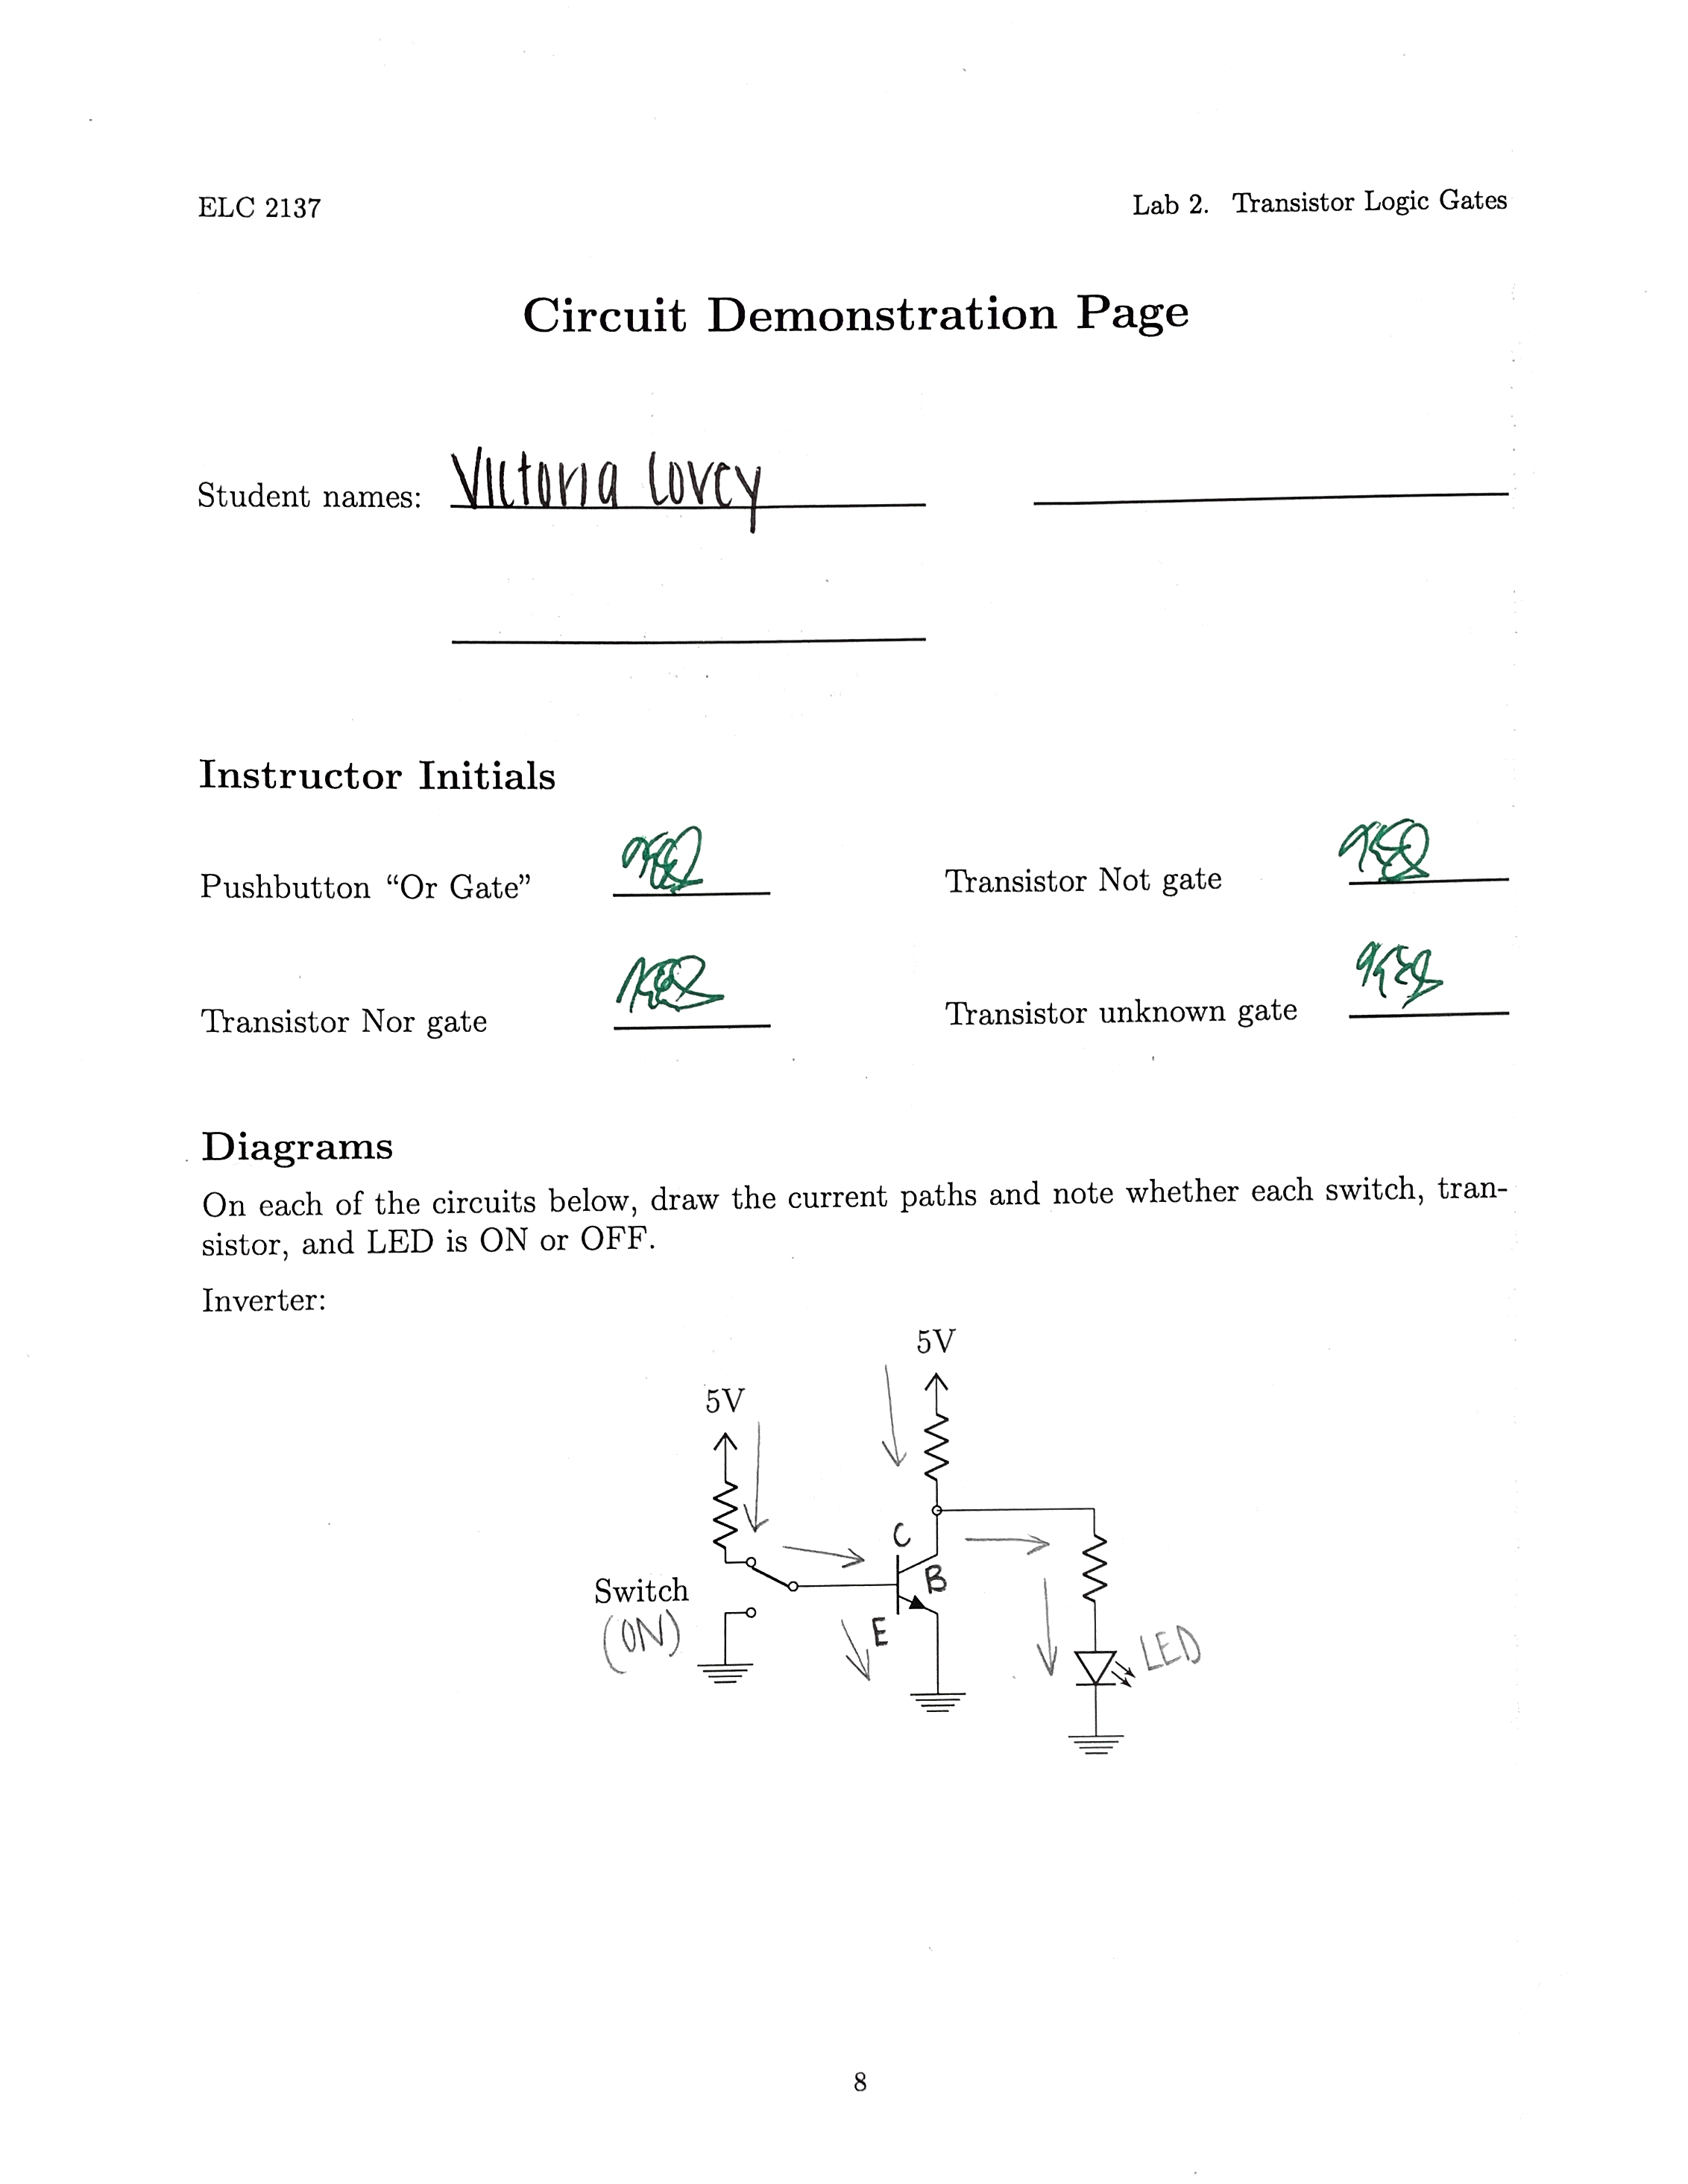
\includegraphics[width=0.8\textwidth,trim=0cm 0cm 0.6cm 0cm,clip]{First_Screenshot}

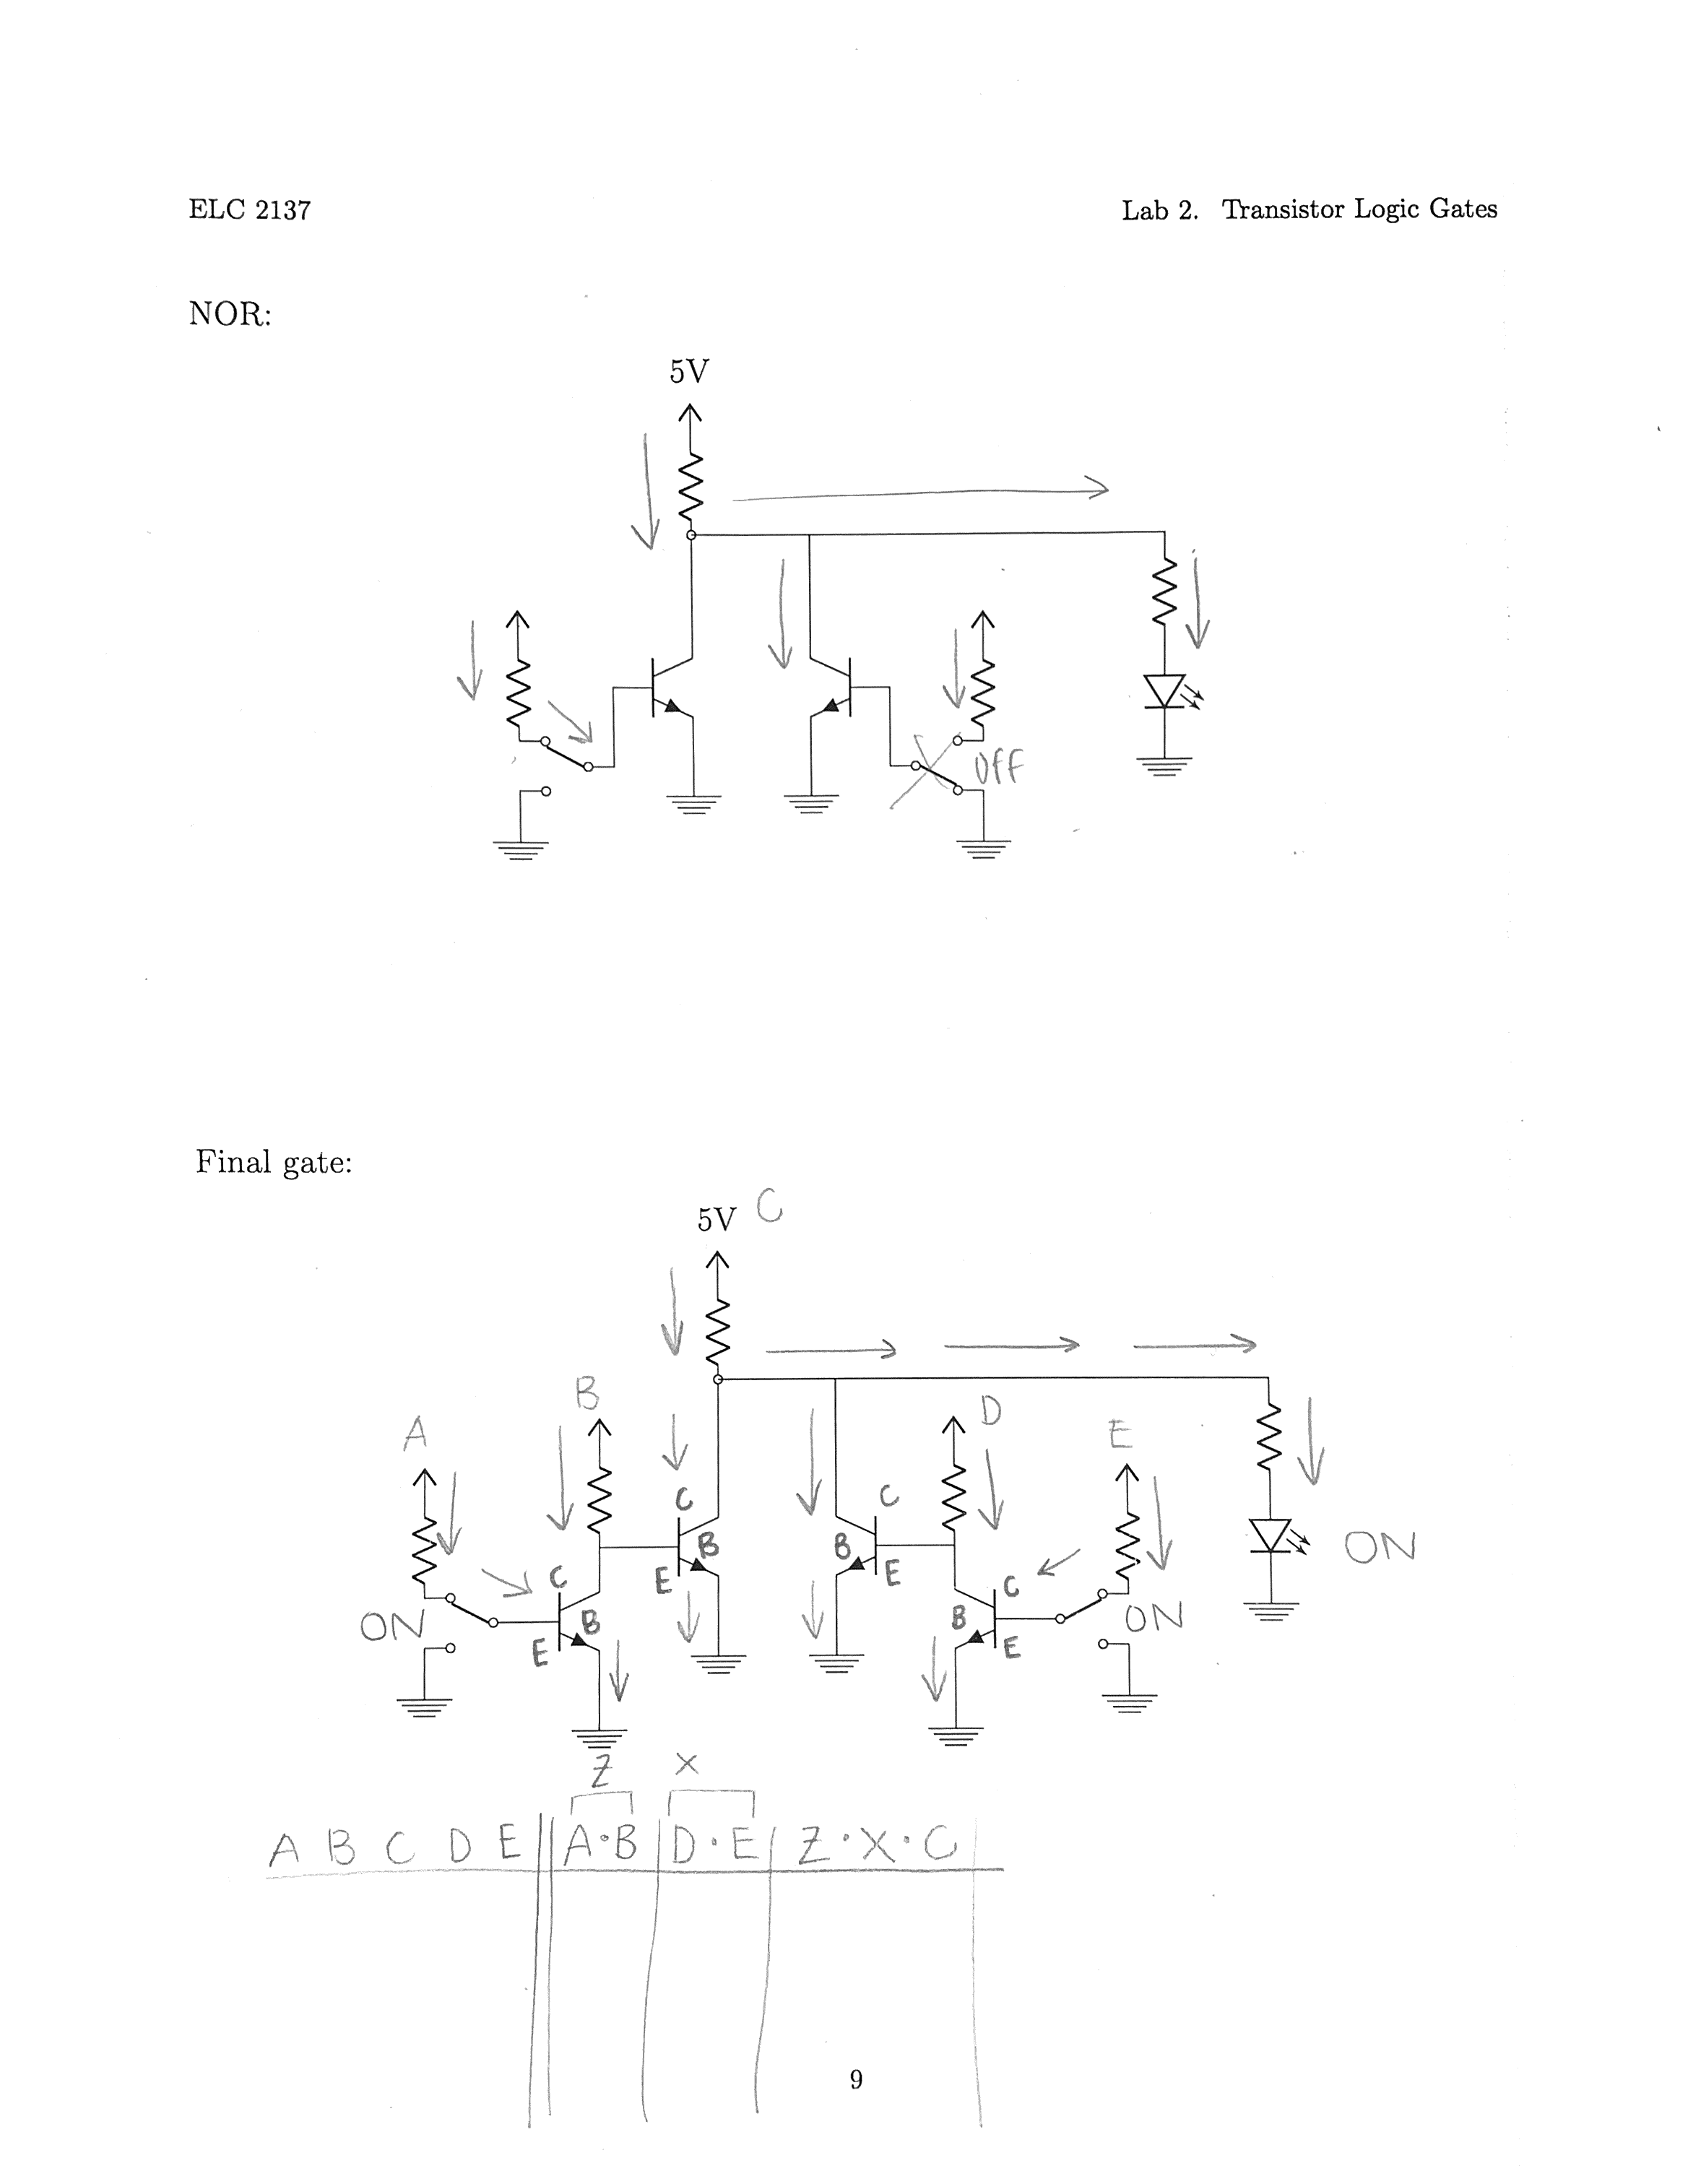
\includegraphics[width=0.8\textwidth,trim=0cm 0cm 0cm 0cm,clip]{Second_SS}

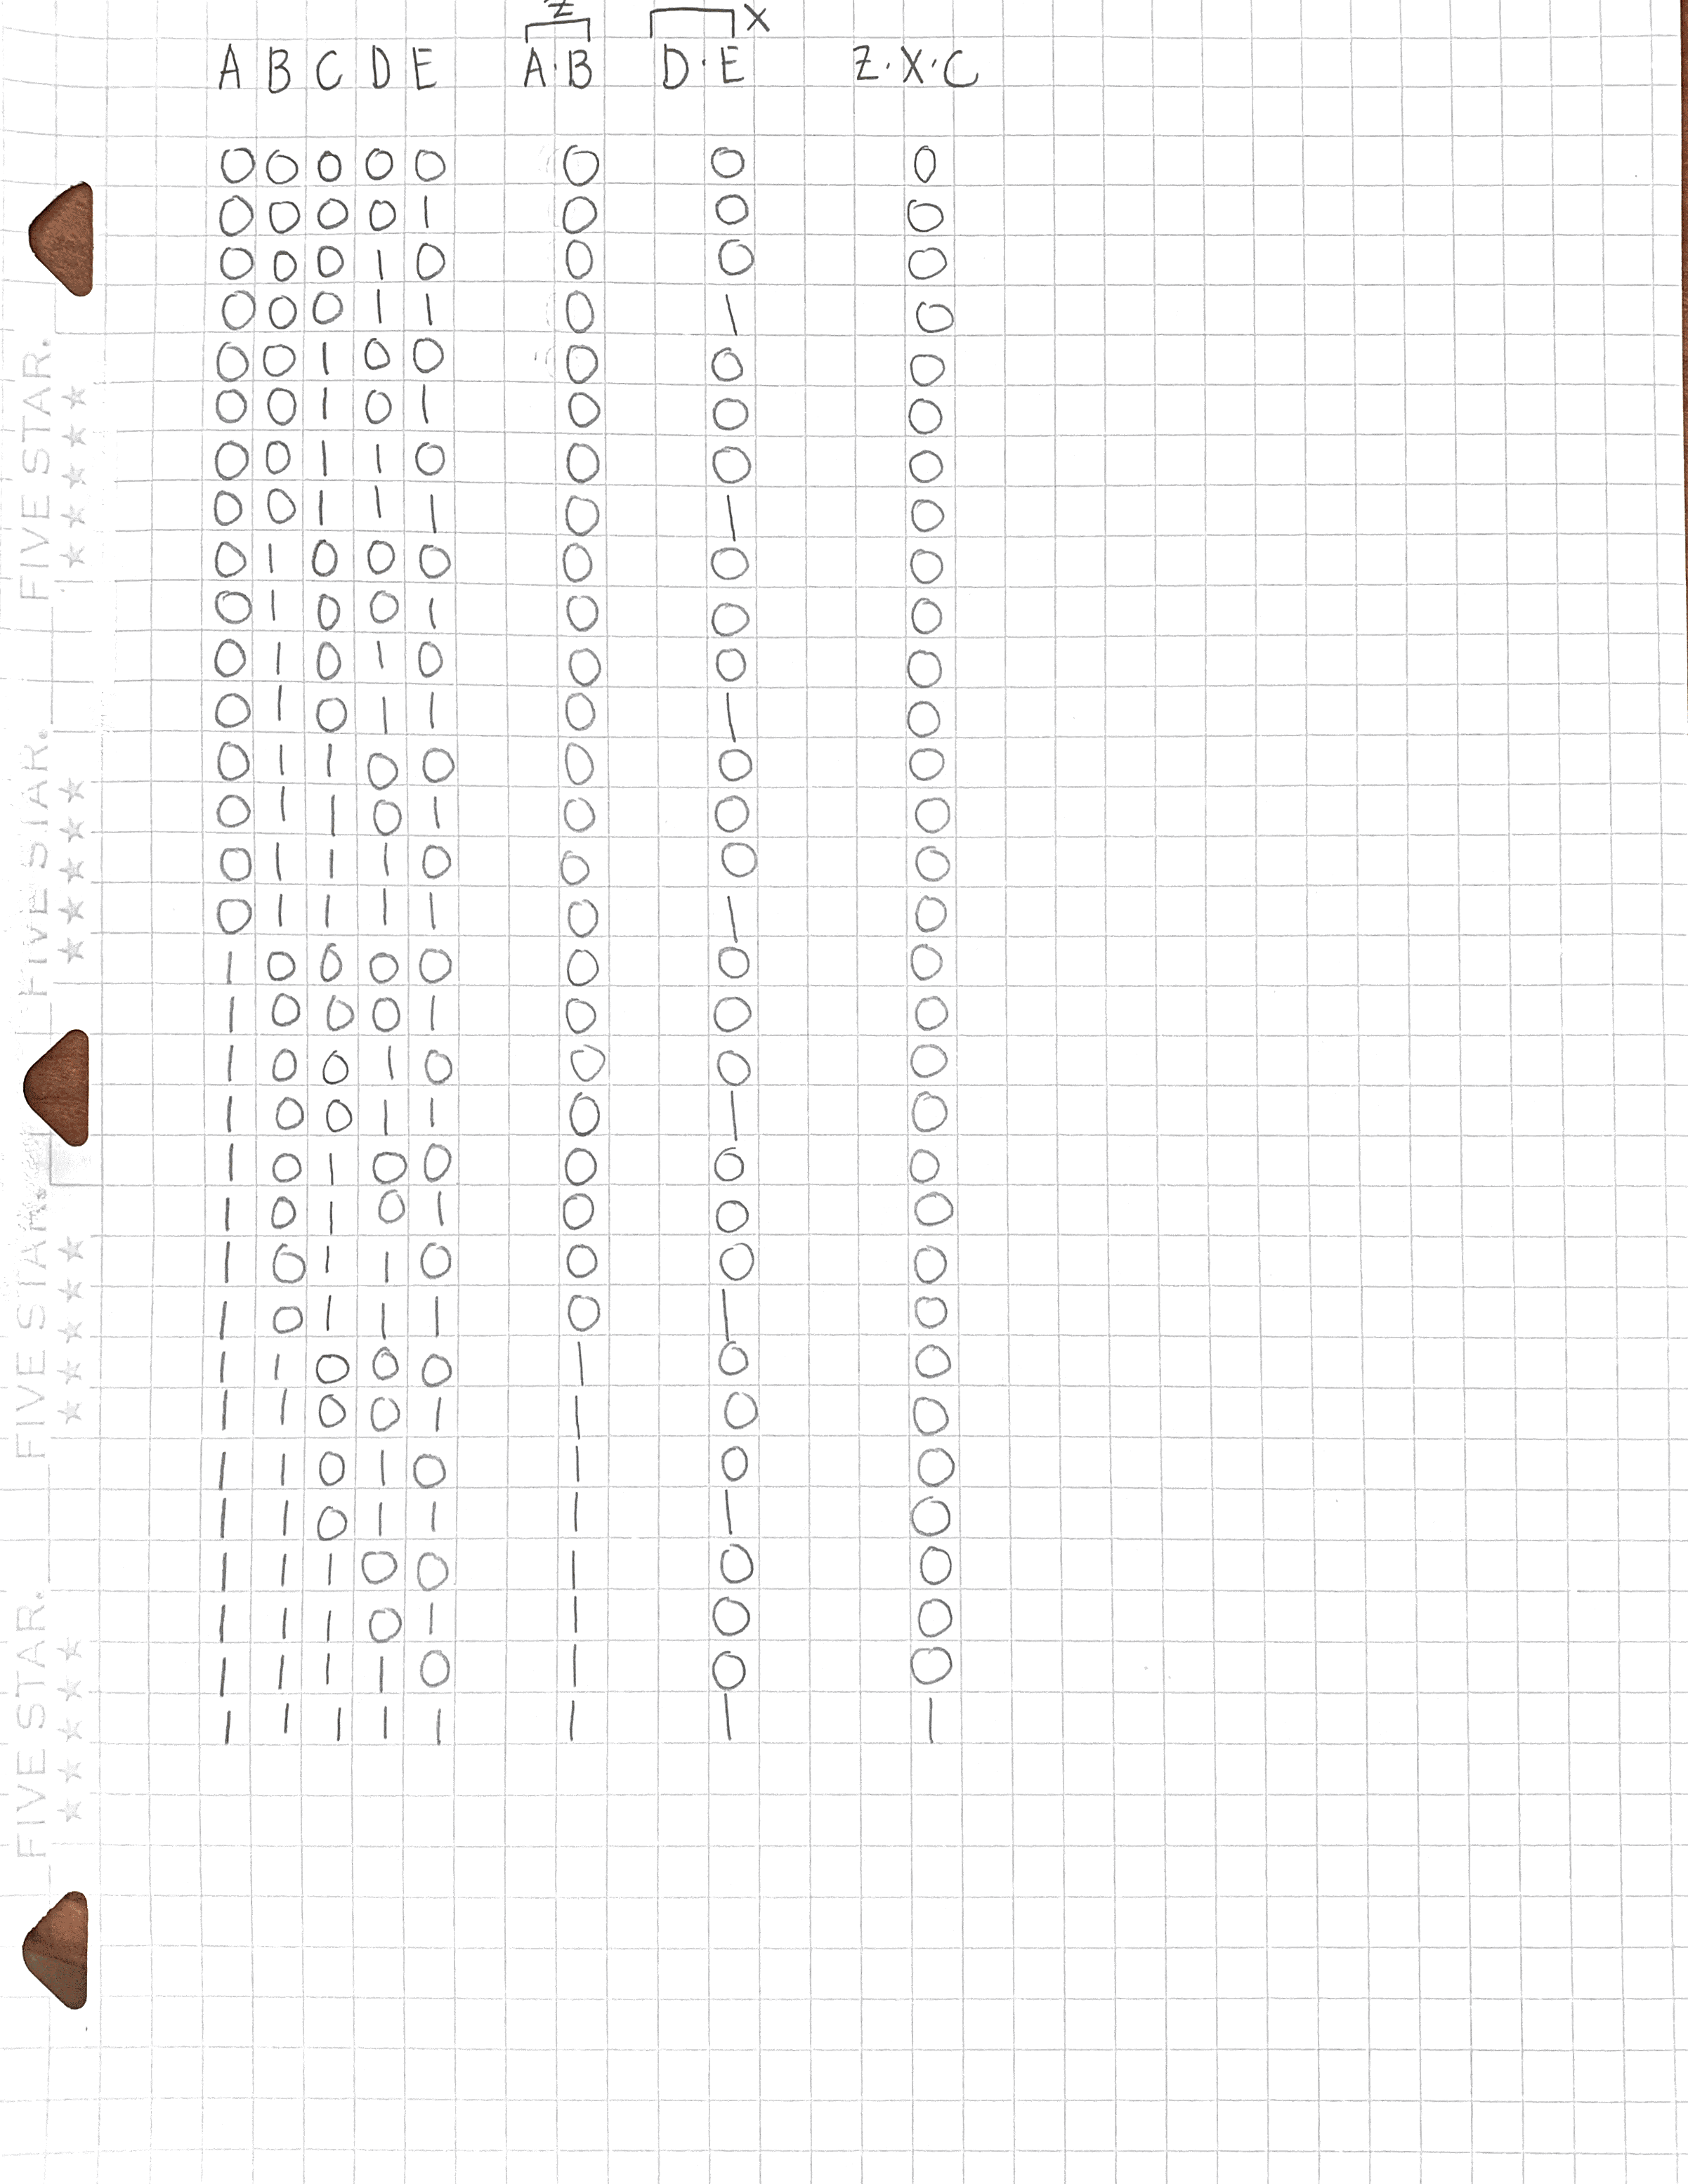
\includegraphics[width=0.8\textwidth,trim=5cm 15cm 15cm 0cm,clip]{Truth_Table}





\end{document}
